\documentclass[answers]{exam}

\renewcommand{\questionlabel}{\textbf{Exercise \thequestion}:}

\usepackage{palatino}
\usepackage{fancyvrb}
\usepackage{amsmath, amssymb, amsfonts}
\usepackage{xcolor}
\usepackage{enumitem}
\setlist[enumerate]{nosep}
\setlist[itemize]{nosep}
\setlist[itemize,1]{label={$\circ$}}
\usepackage{listings}
\lstdefinelanguage{NaBL2}{
  morekeywords={
    module,
    imports,
    signature,
    sorts,
    constructors,
    scope,
    occurrence,
    namespaces,
    name resolution,
    labels,
    order,
    well-formedness,
    constraint generator,
    functions,
    relations,
    reflexive,
    irreflexive,
    symmetric,
    anti-symmetric,
    transitive,
    anti-transitive,
    rules,
    init,
    new,
    true,
    term,
    false,
    error,
    warning,
    note
  },
  otherkeywords={},
  morestring=[b]",
  morecomment=[l]{//},
  morecomment=[n]{/*}{*/},
  literate={...}{$\ldots$}{2},
  mathescape=true,
  escapeinside={`}{`},
  sensitive=true,
}

\lstdefinelanguage{ATerm} {
  morekeywords={},
  otherkeywords={},
  morestring=[b]",
  literate={...}{$\ldots$}2,
  comment=[l]{\%\%},
  mathescape=true,
  escapeinside={`}{`},
  sensitive=true,
}

\lstset{%
  basicstyle={\ttfamily},
  keywordstyle={\bfseries},
  mathescape,
}
\newcommand{\id}[1]{\texttt{#1}}
\newcommand{\pos}[1]{_{\color{gray!130}#1}}
\newcommand{\occ}[2]{\id{#1}\pos{#2}}

%% Package imports
\usepackage{suffix}
\usepackage{relsize}

%% Calculus

\newcommand{\ns}{\mathit{ns}}

%\newcommand{\lbls}{\mathit{labels}}
%\newcommand{\lbl}{\mathit{label}}
%\newcommand{\st}{\mathit{st}}
%\newcommand{\Lbls}{\mathcal{L}}
\newcommand{\Lbl}[1]{\mathbf{#1}}
\newcommand{\RefLbl}{\Lbl{D}}
\newcommand{\DeclLbl}{\Lbl{D}}
%\newcommand{\WF}{\text{WF}}

%\newcommand{\Scopes}{\mathcal{S}}
%\newcommand{\Refs}{\mathcal{R}}
%\newcommand{\Decls}{\mathcal{D}}
%\newcommand{\Edges}{\mathcal{E}}

%\newcommand{\DStep}{\mathbf{D}}
%\newcommand{\EStep}{\mathbf{E}}
%\newcommand{\NStep}{\mathbf{N}}
%\newcommand{\RStep}{\mathbf{R}}

%\newcommand{\reaches}{\rightarrowtail}
%\newcommand{\stepsto}{\rightarrow}
%\WithSuffix\newcommand\stepsto*{\twoheadrightarrow}
%\newcommand{\sees}{\mapsto}
%\newcommand{\resolvesto}{\mapsto}

%\newcommand{\Unknown}{\bot}
%\newcommand{\Total}{\mathsf{T}}
%\newcommand{\Partial}{\mathsf{P}}
%\newcommand{\Res}{\textsc{Res}}
%\newcommand{\Env}{\textsc{Env}}
%\newcommand{\IS}{\textsc{IS}}
%\newcommand{\shadows}{\vartriangleleft}
%\newcommand{\re}{\mathit{re}}

%\newcommand{\rs}{\mathit{rs}}

%%%%%%%%%%%%%%%%%%%%%%%%%%%%%%
%% Graphical Representation %%
%%%%%%%%%%%%%%%%%%%%%%%%%%%%%%

\usepackage{tikz}
\usetikzlibrary{bending,arrows,arrows.meta,shapes,positioning,fit}%

\makeatletter

\newcommand{\fontsizeg}{}

%% Shapes

\newcommand{\sg@occshape}{draw,shape=rectangle}
\newcommand{\sg@scopeshape}{draw,shape=circle}
\newcommand{\sg@varscopeshape}{draw,dashed,shape=circle}
\newcommand{\sg@estepshape}{-{Triangle[length=.5em,angle'=45]}}
\newcommand{\sg@nstepshape}{-{Triangle[length=.5em,angle'=45,open]}}
\newcommand{\sg@typeshape}{-{Square[length=.35em]}}
\newcommand{\sg@resstepshape}{dashed,-{To[length=.5em,angle'=45]}}

%% Inline math commands

\newcommand{\sg@tarrow@impl}[2]{%
  \mathrel{\tikz[baseline=-0.55ex,%
                 thelabel/.style={inner sep=0,pos=.35,text depth=.7em},
                 ]{%
    \draw[line width=.7pt,#1] (0,0) to node[thelabel] {\scalebox{0.6}{$#2$}} (1.5em,0);
  }}%
}
\newcommand{\sg@tarrow}[2]{\begingroup\edef\sg@temp{\endgroup\noexpand\sg@tarrow@impl{#1}{\noexpand#2}}\sg@temp}

\newcommand{\lblt}[1]{\textsf{#1}}
\newcommand{\reflblt}{\lblt{R}}
\newcommand{\decllblt}{\lblt{D}}
\newcommand{\scopelblt}{\lblt{S}}

\newcommand{\refedget}{\sg@tarrow{\sg@estepshape}{}}
\newcommand{\decledget}{\sg@tarrow{\sg@estepshape}{}}
\newcommand{\scopeedget}[1][]{\sg@tarrow{\sg@estepshape}{#1}}
\newcommand{\importedget}[1][]{\sg@tarrow{\sg@nstepshape}{#1}}
\newcommand{\assocedget}[1][]{\sg@tarrow{\sg@nstepshape}{#1}}
\newcommand{\typeedget}{\sg@tarrow{\sg@estepshape}{}}

\newcommand{\occt}[3][]{{}^{\scalebox{0.8}{\textit{#1}}}{#2}_{#3}}
\newcommand{\reft}[3][]{\occt[#1]{#2}{#3}^{\scalebox{0.6}{\reflblt}}}
\newcommand{\declt}[3][]{\occt[#1]{#2}{#3}^{\scalebox{0.6}{\decllblt}}}
\newcommand{\scopet}[1]{#1^{\textsf{\scalebox{0.6}{\scopelblt}}}}

%% Inline graphical commands

\newcommand{\sg@garrow@impl}[3][1.5em]{%
  \tikz[baseline=-0.55ex,
        font={\fontsizeg\sffamily},
        thelabel/.style={inner sep=0,pos=.35,text depth=.7em},
       ]{
    \draw[line width=.7pt,#2] (0,0) to node[thelabel] {\scalebox{0.6}{#3}} (#1,0);
  }%
}
\newcommand{\sg@garrow}[2]{\begingroup\edef\sg@temp{\endgroup\noexpand\sg@garrow@impl{#1}{\noexpand#2}}\sg@temp}

\newcommand{\refedgeg}{\sg@garrow{\sg@estepshape}{}}
\newcommand{\decledgeg}{\sg@garrow{\sg@estepshape}{}}
\newcommand{\scopeedgeg}[1][]{\sg@garrow{\sg@estepshape}{#1}}
\newcommand{\importedgeg}[1][]{\sg@garrow{\sg@nstepshape}{#1}}
\newcommand{\assocedgeg}[1][]{\sg@garrow{\sg@nstepshape}{#1}}
\newcommand{\resedgeg}[1][]{\sg@garrow{\sg@resstepshape}{#1}}
\newcommand{\typeedgeg}[1][]{\sg@garrow{\sg@typeshape}{#1}}

\newcommand{\sg@node@impl}[2]{%
  \tikz[baseline=-0.55ex,
        font=\fontsizeg,
        thenode/.style = {minimum width=1.3em, minimum height=1.3em,
                          inner xsep=.1em, inner ysep=0, outer sep=0,
                          text depth=0, text height=.5em},
       ]{
    \node[thenode,#1] (enclosing) {\smash{$#2$}};
  }%
}
\newcommand{\sg@node}[2]{\begingroup\edef\sg@temp{\endgroup\noexpand\sg@node@impl{#1}{\noexpand#2}}\sg@temp}

\newcommand{\occg}[3][]{\sg@node{\sg@occshape}{\occt[#1]{#2}{#3}}}
\let\refg\occg
\let\declg\occg
\newcommand{\scopeg}[1]{\sg@node{\sg@scopeshape}{#1}}
\newcommand{\varscopeg}[1]{\sg@node{\sg@varscopeshape}{#1}}

\makeatother

%% Tikz styles

\tikzset{%
  scopegraph/.style = {%
    %% node styles
    every node/.style = {draw, minimum size=1.5em},
    scope/.style = {shape=circle},
    varscope/.style = {scope, dashed},
    occurrence/.style = {shape=rectangle},
    decl/.style = {occurrence},
    ref/.style = {occurrence},
    superscript label/.style = {},%
    superscript/.style={label={[superscript label,minimum size=0,inner sep=.2ex]45:{\smaller[2]\textit{##1}}}},%
    %% arrow styles
    direct arrow/.style = {-{Triangle[length=.5em,angle'=60,flex']}},
    named arrow/.style = {-{Triangle[length=.5em,angle'=60,open,flex']}},
    importref arrow/.style = {{Triangle[length=.5em,angle'=60,flex']}-{Triangle[length=.5em,angle'=60,open,flex']}},
    resolve arrow/.style = {-{To[length=.5em,angle'=60,flex']}},
    type arrow/.style = {-{Square[length=.35em,flex']}},
    %% edge styles
    every edge/.style = {draw, direct arrow},
    import/.style = {named arrow},
    export/.style = {named arrow},
    type/.style = {type arrow},
    importref/.style = {importref arrow},%
    resolve/.style = {dashed, resolve arrow, shorten <= .2em, shorten >= .2em},%
    lbl/.style = {edge node = {node[draw=none,fill=white,minimum size=0,inner sep=.2ex, pos=.45] {\smaller[2]\textsf{##1}}}},%
  },%
}

\tikzset{scopegraph/.append style = {
  decl/.append style = {fill=olive!50},
  ref/.append style = {fill=gray!30},
}}

\pagestyle{headandfoot}

\header{\textsf{IN4303: Compiler Construction}}{\textsf{\textsc{Exercises}}}{\textsf{Oct 24, 2017}}
\headrule

\footer{}{\textsf{Page \thepage{} of \numpages}}{}
\footrule

\begin{document}

\begin{questions}

  \question Name Resolution
  \begin{parts}
    \part Explain the main aspects of name resolution with scope graphs.

    \begin{solution}
      The main aspects are:
      \begin{itemize}
      \item The name binding structure of a program is represented as
        a graph of scopes, references, and declarations.
      \item Resolving a reference is finding a path in the graph from
        the reference to a matching declaration.
      \item The paths used for resolution must be well-formed, which
        means the labels must match a given well-formedness regular
        expression.
      \item Disambiguation defines which declarations are visible if
        multiple matching declarations can be reached. Disambiguation
        is specified using an ordering on path labels.
      \end{itemize}
    \end{solution}

    \part Given the following scope graph, list all reachability paths
    for reference $\occ{A}{6}$. Also indicate the path that is chosen
    according to the visibility rules.

    \begin{center}
      \begin{tikzpicture}[scopegraph]
        \node[scope] (s0) {$0$};
        \node[decl, above = of s0.center] (A7) {$\occ{A}{7}$};
        \node[decl, above right = of s0.center] (M1) {$\occ{M}{1}$};
        \node[scope, right = of M1.center] (s1) {$1$};
        \node[decl, right = of s1.center] (A2) {$\occ{A}{2}$};
        \node[ref, left = of s0.center] (Q5) {$\occ{Q}{5}$};
        \node[scope, below = of Q5.center] (s3) {$3$};
        \node[ref, right = of s3.center] (A6) {$\occ{A}{6}$};
        \node[decl, below right = of s0.center] (Q3) {$\occ{Q}{3}$};
        \node[scope, right = of Q3.center] (s2) {$2$};
        \node[ref, right = of s2.center] (M4) {$\occ{M}{4}$};

        \draw (s0) edge (A7);
        \draw (s0) edge[out=30, in=190] (M1);
        \draw (Q5) edge (s0);
        \draw (s3) edge[import, left, lbl={I}] (Q5);
        \draw (A6) edge (s3);
        \draw (M1) edge[export, lbl={I}] (s1);
        \draw (s0) edge[out=-30, in=170] (Q3);
        \draw (Q3) edge[export, lbl={I}] (s2);
        \draw (s1) edge[lbl={P}, bend left=15] (s0);
        \draw (s1) edge (A2);
        \draw (s2) edge[import, lbl={I}, bend right] (M4);
        \draw (M4) edge[bend right] (s2);
        \draw (s2) edge[lbl={P}, bend right=15] (s0);

        \ifprintanswers
        \draw (A6) edge[resolve, above, lbl={R}, bend right] (s3);
        \draw (s3) edge[resolve, below, lbl={I($\occ{Q}{5}$)}, bend right] (s2);
        \draw (s2) edge[resolve, right, lbl={I($\occ{M}{4}$)}] (s1);
        \draw (s1) edge[resolve, above, lbl={D}, bend left] (A2);
        \fi
      \end{tikzpicture}
    \end{center}

    \begin{solution}
      There is one reachable path for $\occ{A}{6}$, which is shown
      with the dashed arrows in the figure above. The path is
      well-formed, since its labels \lblt{I}\lblt{I} match the
      well-formedness $\lblt{P}^\ast \lblt{I}^\ast$. Becasue there is
      only one reachable declaration, it is also the visible
      declaration.
    \end{solution}

    \part Given the following Java program,
    \begin{lstlisting}[language=Java,gobble=6]
      public class A$\pos{1}$ {
        int f$\pos{2}$;
      }

      public class B$\pos{3}$ {
        int m$\pos{4}$(A$\pos{5}$ o$\pos{6}$) {
          return o$\pos{7}$.f$\pos{8}$;
        }
      }
    \end{lstlisting}
    give a scope graph that describes its name binding structure. Use
    the subscripts on identifiers to distinguish different occurrences
    of the same name. For the type-dependent field name, you also need
    to list the constraints that are necessary.

    \begin{solution}
      The scope graph and constraints for the program are given by:
      \begin{center}
        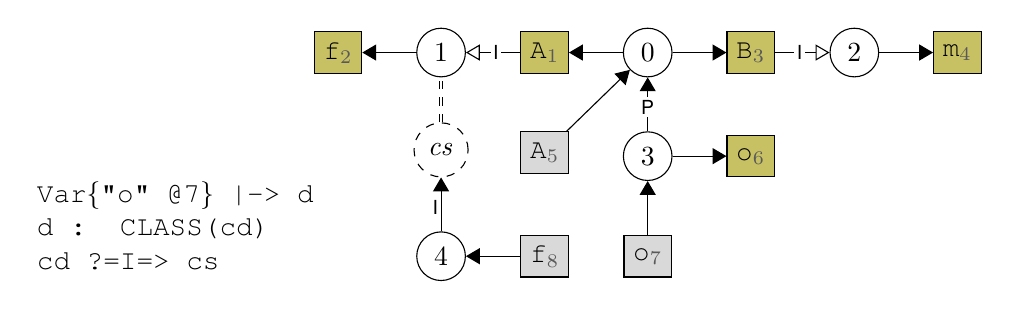
\begin{tikzpicture}[scopegraph]
          \node[scope] (s0) {$0$};

          \node[decl, left = of s0.center] (A1) {$\occ{A}{1}$};
          \draw (s0) edge (A1);
          \node[scope, left = of A1.center] (s1) {$1$};
          \draw (A1) edge[export, lbl={I}] (s1);
          \node[decl, left = of s1.center] (f2) {$\occ{f}{2}$};
          \draw (s1) edge (f2);

          \node[decl, right = of s0.center] (B3) {$\occ{B}{3}$};
          \draw (s0) edge (B3);
          \node[scope, right = of B3.center] (s2) {$2$};
          \draw (B3) edge[export, lbl={I}] (s2);
          \node[decl, right = of s2.center] (m4) {$\occ{m}{4}$};
          \draw (s2) edge (m4);

          \node[ref, below left = of s0.center] (A5) {$\occ{A}{5}$};
          \draw (A5) edge (s0);
          \node[scope, below = of s0.center] (s3) {$3$};
          \draw (s3) edge[lbl={P}] (s0);
          \node[decl, right = of s3.center] (o6) {$\occ{o}{6}$};
          \draw (s3) edge (o6);

          \node[ref, below = of s3.center] (o7) {$\occ{o}{7}$};
          \draw (o7) edge (s3);

          \node[ref, below left = of s3.center] (f8) {$\occ{f}{8}$};
          \node[scope, left = of f8.center] (s4) {$4$};
          \draw (f8) edge (s4);
          \node[varscope, above = of s4.center] (cs) {$\mathit{cs}$};
          \draw (s4) edge[left, lbl={I}] (cs);
          \draw (cs) edge[-,dashed,double] (s1);

          \node[draw=none, font={\ttfamily}, every text node part/.style={align=left}] (C) at (-6,-2.2) {
            Var\{"o" @7\} |-> d \\
            d : CLASS(cd) \\
            cd ?=I=> cs
          };
        \end{tikzpicture}
      \end{center}
      Note that we kept the scope variable \textit{cs} explicit in the
      graph, and indicated the substitution with the double dashed
      line. This makes it easier to make the connection with the
      constraints, than if scope $4$ was directly connected to scope
      $1$.
    \end{solution}
  \end{parts}

  \question Typing Constraints
  \begin{parts}
    \part Explain the main aspects of type checking with
    constraints. Discuss how the different parts of your answer are
    related to the language the checker is for.

    \begin{solution}
      Type checking with constraints is based on the idea that the
      property of well-typedness of a program can be stated as a
      constraint problem. If the constraint problem is satisfied, the
      program is well-typed. This is implemented in two phases:
      \begin{enumerate}
      \item Constraint \emph{generation} maps the program to a
        constraint problem. This step is language-dependent,
        constraint generation rules are defined over the syntax of the
        language.
      \item Constraint \emph{solving} checks if the constraint problem
        is satisfiable, and tries to find values for the constraint
        variables. Constraint solving depends only on the constraint
        language, but is independent of the object language that is
        being checked.
      \end{enumerate}
    \end{solution}

    \part Explain the concepts of soundness and completeness in terms
    of your previous answer.

    \begin{solution}
      Soundness and completeness are properties that relate the
      semantics of constraints to the solver algorithm.

      Soundness means that any answer the solver gives, is indeed a
      valid solution to the constraints, according to the constraint
      semantics. In the context of type checking, this means that if a
      program is ill-typed, the equivalent constraint problem must be
      unsatisfiable, and the solver reports an error that it cannot
      find a valid solution.

      Completeness means that if a valid solution exists, the solver
      finds it. In the context of type checking, this means that if a
      program is well-typed, the constraint problem is satisfiable,
      and the solver returns a valid solution, i.e. a valid
      assignments for all the constraint variables.
    \end{solution}

    \part\label{unify} Given the following type equalities,
    \begin{Verbatim}[gobble=6]
      f(a) == b, g(b,d) == g(f(c),f(e)), h() == e
    \end{Verbatim}
    give a substitution that satisfies the equalities.

    \begin{solution}
      A possible unifying substitution is:
      \begin{align*}
        a &\mapsto c & b &\mapsto \texttt{f($c$)} & d &\mapsto \texttt{f(h())} & e &\mapsto \texttt{h()}
      \end{align*}
    \end{solution}

    \part Explain the concept of principality in terms of your
    previous answer. Illustrate your answer with a different unifier
    that would also satisfy the constraints of (\ref{unify}).

    \begin{solution}
      A given substitution $s$ is a principal unifier if every other
      unifier $s'$ is an instance of $s$. A unifier $s'$ is an
      instance of $s$ if a substitution $s''$ exists, such that $s''$
      applied to $s$ yields $s$.

      In the example, any substitution that fixes a term value $t$ for
      $c$ is still a unifier for the constraints. However, it would
      not be principal anymore. The substitution $s''$ in this
      scenario would be given by $s \mapsto t$.

      Possible additions:
      \begin{itemize}
      \item Principal unifiers are not necessarily unique. For
        example, the variables $a$ and $c$ could be swapped in our
        example solution and it would remain principle.
      \item In type systems there is a similar concept: principle
        types. These are types that are supertypes of all other valid
        types for a program. For example, the identity function
        \lstinline[language=Haskell]!\x -> x! may have type
        \lstinline[language=Haskell]!Int -> Int! or
        \lstinline[language=Haskell]!String -> String!, but its
        principal type is \lstinline[language=Haskell]!forall a. a -> a!.
      \end{itemize}
    \end{solution}
  \end{parts}

  \question Constraint Semantics

  Consider the constraint $d : t$ that gives the type $t$ of a
  declaration $d$. The semantic rule for this constraint is given by
  \[
    T, G, s \vDash d : t \qquad \text{where } T(s(d)) = s(t)
  \]
  where $T : \mathit{Decl} \to \mathit{Type}$ is a function from types
  to declarations, $G$ is a scope graph, and $s$ is a variable
  substitution.

  \begin{parts}
    \part Given the constraints
    \begin{Verbatim}[gobble=6]
      Var{“a” @1} : ty1, ty1 == INT(), Var{“a” @1} : ty2
    \end{Verbatim}
    give a substitution $s$ for the variables \textit{ty1} and
    \textit{ty2}, such that the constraints are \emph{not}
    satisfiable, according to the semantic rule given above.

    \begin{solution}
      The substitution
      \begin{align*}
        \mathit{ty1} &\mapsto \texttt{INT()} & \mathit{ty2} &\mapsto \texttt{STRING()}
      \end{align*}
      cannot satisfy the constraints. The function $T$ enforces that
      every declaration has only one type. If we pick
      $T(\texttt{Var\{a @1\}}) = \texttt{INT()}$, the third constraint
      is unsatisfiable. If we pick
      $T(\texttt{Var\{a @1\}}) = \texttt{STRING()}$, the first
      constraint is unsatisfiable. If we pick any other value, both
      will be unsatisfiable.
    \end{solution}

    \part We use \texttt{type-of(d, ty)} as the textual representation
    of $d : t$ constraints. The following rule specifies a possible
    solver for \texttt{type-of} constraints:
    \begin{Verbatim}[gobble=6]
      type-of(d,ty1), type-of(d, ty2) <=> ty1 == ty2.
    \end{Verbatim}

    Show using a counter-example that this rule is unsound. Explain
    how the rule is applied in your example.

    \begin{solution}
      The following constraints (for some declaration $d$) are a
      counter example:
      \begin{Verbatim}[gobble=8]
        type-of(d, INT()), type-of(d, STRING()), type-of(d, INT())
      \end{Verbatim}
      The constraints specify two different types for the
      declaration. Therefore, the solver should not be able to solve
      these constraints. To show this rule is unsound, we need to show
      a derivation that accepts these constraints. A possible
      derivation is:
      \begin{Verbatim}[gobble=6]
            type-of(d, INT()), type-of(d, STRING()), type-of(d, INT())
        <=> type-of(d, STRING()), INT() == INT()
        <=> type-of(d, STRING())
      \end{Verbatim}
      The first step applies the given rule to the first and last
      constraint, simplifying it to an equality. The second step
      discharges the equality, which is obviously satisfied. Since no
      more rules can be applied, the solver concludes the constraint
      problem is satisfied.
    \end{solution}

    \part Modify the rule above to make it sound, and explain why your
    counter-example is now rejected.

    \begin{solution}
      A sound version of the rule is
      \begin{Verbatim}[gobble=8]
        type-of(d,ty1), type-of(d, ty2) <=> type-of(d, ty1), ty1 == ty2.
      \end{Verbatim}
      Instead of checking consistency only between pairs, we now check
      consistency of all constraints. For example, the derivation we
      had before will now look as follows:
      \begin{Verbatim}[gobble=6]
            type-of(d, INT()), type-of(d, STRING()), type-of(d, INT())
        <=> type-of(d, INT()), type-of(d, STRING()), INT() == INT()
        <=> type-of(d, INT()), type-of(d, STRING())
        <=> INT() == STRING()
        <=> false
      \end{Verbatim}
      Now the solver ends with an equality that cannot be satisfied,
      and the problem is reported as unsatisfiable.
    \end{solution}
  \end{parts}

  \question Constraint Rules
  \begin{parts}
    \part\label{generate} Given the following constraint rules
    \begin{lstlisting}[language=NaBL2,gobble=6]
      [[ LetRec(binds) ^ (s) : ty ]] :=
        new s_let, s_let ---> s,
        Map1[[ binds ^ (s_let) ]],
        [[ e ^ (s_let) : ty ]].

      [[ Bind(x, e) ^ (s) ]] :=
        Var{x} <- s, Var{x} : ty,
        [[ e ^ (s) : ty ]].

      [[ IntLit(_) ^ (s) : INT() ]].

      [[ VarRef(x) ^ (s) : ty ]] :=
        Var{x} -> s, Var{x} |-> d, d : ty. 
    \end{lstlisting}
    and the program represented by the following abstract syntax tree,
    \begin{lstlisting}[language=ATerm,gobble=6]
      LetRec([
        Bind("x"$\pos{1}$,IntLit(42)), 
        Bind("y"$\pos{2}$,VarRef("x"$\pos{3}$)),
      ], VarRef("y"$\pos{4}$))
    \end{lstlisting}
    show the constraints that would be generated by applying these
    rules to the program. Feel free to rename variables if necessary
    to avoid capture.

    \begin{solution}
      Step by step application of the rules  to the program gives:
      \begin{lstlisting}[language=NaBL2, basicstyle={\footnotesize\ttfamily}, gobble=8]
           [[ LetRec([Bind("x"$\pos{1}$,IntLit(42)),Bind("y"$\pos{2}$,VarRef("x"$\pos{3}$))],VarRef("y"$\pos{4}$)) ^ (s) : ty ]]
        => new s_let, s_let ---> s,
           Map1[[ [Bind("x"$\pos{1}$,IntLit(42)),Bind("y"$\pos{2}$,VarRef("x"$\pos{3}$))] ^ (s_let) : ty ]],
           [[ VarRef("y"$\pos{4}$) ^ (s_let) : ty ]]
        => new s_let, s_let ---> s,
           [[ Bind("x"$\pos{1}$,IntLit(42)) ^ (s_let) ]],
           [[ Bind("y"$\pos{2}$,VarRef("x"$\pos{3}$)) ^ (s_let) ]],
           [[ VarRef("y"$\pos{4}$) ^ (s_let) : ty ]]
        => new s_let, s_let ---> s,
           Var{"x"$\pos{1}$} <- s_let, Var{"x"$\pos{1}$} : ty1, [[ IntLit(42) ^ (s_let) : ty1 ]],
           [[ Bind("y"$\pos{2}$,VarRef("x"$\pos{3}$)) ^ (s_let) ]],
           [[ VarRef("y"$\pos{4}$) ^ (s_let) : ty ]]
        => new s_let, s_let ---> s,
           Var{"x"$\pos{1}$} <- s_let, Var{"x"$\pos{1}$} : ty1, ty1 == INT(),
           [[ Bind("y"$\pos{2}$,VarRef("x"$\pos{3}$)) ^ (s_let) ]],
           [[ VarRef("y"$\pos{4}$) ^ (s_let) : ty ]]
        => new s_let, s_let ---> s,
           Var{"x"$\pos{1}$} <- s_let, Var{"x"$\pos{1}$} : ty1, ty1 == INT(),
           Var{"y"$\pos{2}$} <- s_let, Var{"y"$\pos{2}$} : ty2, [[ VarRef("x"$\pos{3}$) ^ (s_let) : ty2 ]].
           [[ VarRef("y"$\pos{4}$) ^ (s_let) : ty ]]
        => new s_let, s_let ---> s,
           Var{"x"$\pos{1}$} <- s_let, Var{"x"$\pos{1}$} : ty1, ty1 == INT(),
           Var{"y"$\pos{2}$} <- s_let, Var{"y"$\pos{2}$} : ty2, Var{"x"$\pos{3}$} -> s_let, Var{"x"$\pos{3}$} |-> d1, d1 : ty2,
           [[ VarRef("y"$\pos{4}$) ^ (s_let) : ty ]]
        => new s_let, s_let ---> s,
           Var{"x"$\pos{1}$} <- s_let, Var{"x"$\pos{1}$} : ty1, ty1 == INT(),
           Var{"y"$\pos{2}$} <- s_let, Var{"y"$\pos{2}$} : ty2, Var{"x"$\pos{3}$} -> s_let, Var{"x"$\pos{3}$} |-> d1, d1 : ty2,
           Var{"y"$\pos{4}$} -> s_let, Var{"y"$\pos{4}$} |-> d2, d2 : ty
      \end{lstlisting}
    \end{solution}

    \part Give a solution for the constraints you generated in
    (\ref{generate}), or explain why a solution is not possible.

    \begin{solution}
      A solution must consists of all the components of the constraint
      semantics: a scope graph $G$, a typing function $T$, and a
      substitution $s$. The substitution $s$ is given by:
      \begin{align*}
        \mathit{s_\text{let}} &\mapsto \scopeg{1} \\
        \mathit{ty} &\mapsto \texttt{INT()} \\
        \mathit{ty1} &\mapsto \texttt{INT()} \\
        \mathit{ty2} &\mapsto \texttt{INT()} \\
        \mathit{d1} &\mapsto \texttt{Var{"x"$\pos{1}$}} \\
        \mathit{d2} &\mapsto \texttt{Var{"y"$\pos{2}$}}
      \end{align*}
      The declarations to types function $T$ is given by:
      \begin{align*}
        \texttt{Var\{"x"$\pos{1}$\}} &: \texttt{INT()} \\
        \texttt{Var\{"y"$\pos{2}$\}} &: \texttt{INT()}
      \end{align*}
      The scope graph $G$ is given by:
      \begin{center}
        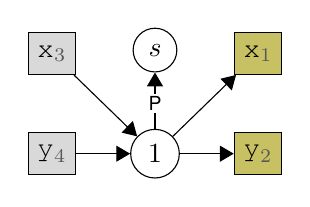
\begin{tikzpicture}[scopegraph]
          \node[scope] (s) {$s$};
          \node[scope, below = of s.center] (s1) {$1$};
          \draw (s1) edge[lbl={P}] (s);

          \node[decl, above right = of s1.center] (x1) {$\occ{x}{1}$};
          \draw (s1) edge (x1);
          \node[decl, right = of s1.center] (y2) {$\occ{y}{2}$};
          \draw (s1) edge (y2);
          \node[ref, above left = of s1.center] (x3) {$\occ{x}{3}$};
          \draw (x3) edge (s1);
          \node[ref, left = of s1.center] (y4) {$\occ{y}{4}$};
          \draw (y4) edge (s1);
        \end{tikzpicture}
      \end{center}
    \end{solution}

    \part The rules from (\ref{generate}) model a recursive let. An
    alternative semantics for let, where the bodies of the bindings
    cannot refer to the variables that are defined in the let, but
    only to variables defined outside the let. Give a set of modified
    rules that implement these let semantics.

    \begin{solution}
      Only the rules for let and bind have to be changed. The rules
      are changed in such a way that the expressions in the binds are
      not checked in the let scope, but in the surrounding lexical
      scope. These are the rules for parallel lets:
      \begin{lstlisting}[language=NaBL2,gobble=8]
        [[ LetRec(binds) ^ (s) : ty ]] :=
          new s_let, s_let ---> s,
          Map1[[ binds ^ (s, s_let) ]],
          [[ e ^ (s_let) : ty ]].

        [[ Bind(x, e) ^ (s, s_let) ]] :=
          Var{x} <- s_let, Var{x} : ty,
          [[ e ^ (s) : ty ]].
      \end{lstlisting}
    \end{solution}
  \end{parts}
  
\end{questions}

\end{document}